%%%%%%%%%%%%%%%%%%%%%%%%%%%%%%%%%%%%%%%%%%%%%%%%%%%%%%%%%%%%%%%%%%%%%%%%%%%%%%%%
%%%%%%%%%%%%%%%%%%%%%%%%%%%%%%%%%%%%%%%%%%%%%%%%%%%%%%%%%%%%%%%%%%%%%%%%%%%%%%%%
%%                                                                            %%
%% thesistemplate.tex version 3.01 (2017/10/06)                               %%
%% The LaTeX template file to be used with the aaltothesis.sty (version 3.01) %%
%% style file.                                                                %%
%%                                                                            %%
%% This is licensed under the terms of the MIT license below.                 %%
%%                                                                            %%
%% Copyright 2017, by Luis R.J. Costa, luis.costa@aalto.fi,                   %%
%% Copyright 2017 documentation in Finnish in the template by Perttu Puska,   %%
%% perttu.puska@aalto.fi                                                      %%
%% Copyright Swedish translations 2014 by Elisabeth Nyberg,                   %%
%% elisabeth.nyberg@aalto.fi and Henrik Wallén, henrik.wallen@aalto.fi        %%
%%                                                                            %%
%% Permission is hereby granted, free of charge, to any person obtaining a    %%
%% copy of this software and associated documentation files (the "Software"), %%
%% to deal in the Software without restriction, including without limitation  %%
%% the rights to use, copy, modify, merge, publish, distribute, sublicense,   %%
%% and/or sell copies of the Software, and to permit persons to whom the      %%
%% Software is furnished to do so, subject to the following conditions:       %%
%% The above copyright notice and this permission notice shall be included in %%
%% all copies or substantial portions of the Software.                        %%
%% THE SOFTWARE IS PROVIDED "AS IS", WITHOUT WARRANTY OF ANY KIND, EXPRESS OR %%
%% IMPLIED, INCLUDING BUT NOT LIMITED TO THE WARRANTIES OF MERCHANTABILITY,   %%
%% FITNESS FOR A PARTICULAR PURPOSE AND NONINFRINGEMENT. IN NO EVENT SHALL    %%
%% THE AUTHORS OR COPYRIGHT HOLDERS BE LIABLE FOR ANY CLAIM, DAMAGES OR OTHER %%
%% LIABILITY, WHETHER IN AN ACTION OF CONTRACT, TORT OR OTHERWISE, ARISING    %%
%% FROM, OUT OF OR IN CONNECTION WITH THE SOFTWARE OR THE USE OR OTHER        %%
%% DEALINGS IN THE SOFTWARE.                                                  %%
%%                                                                            %%
%%                                                                            %%
%%%%%%%%%%%%%%%%%%%%%%%%%%%%%%%%%%%%%%%%%%%%%%%%%%%%%%%%%%%%%%%%%%%%%%%%%%%%%%%%
%%%%%%%%%%%%%%%%%%%%%%%%%%%%%%%%%%%%%%%%%%%%%%%%%%%%%%%%%%%%%%%%%%%%%%%%%%%%%%%%

%\documentclass[english, 12pt, a4paper, elec, utf8, pdfa]{aaltothesis}
\documentclass[english, 12pt, a4paper, elec, utf8, pdfa, online]{aaltothesis}
%\documentclass[english,12pt,a4paper,dvips]{aaltothesis}

\newcommand{\pubdate}{<Publish date>}
%% Use the following options in the \documentclass macro above:
%% your school: arts, biz, chem, elec, eng, sci
%% the character encoding scheme used by your editor: utf8, latin1
%% thesis language: english, finnish, swedish
%% make an archiveable PDF/A compatible file: pdfa
%% symmetric typeset layout and blue hypertext for online publication: online
%%            (no option is the default, resulting in a wide margin on the
%%             binding side of the page and black hypertext)
%% two-sided printing: twoside (default is one-sided printing)
%%

\usepackage{graphicx}
\usepackage{cite}
\usepackage{amsfonts,amssymb,amsbsy}

\usepackage{listings}
\definecolor{commentgreen}{rgb}{0,0.5,0}
\lstset {
    basicstyle=\ttfamily,
    texcl=true,
    tabsize=4,
    keywordstyle=\color{blue},
    commentstyle=\color{commentgreen},
    identifierstyle=\color{black},
    stringstyle=\color{red},
    breaklines=true,
    numbers=left,
    numberstyle={\small \color{black}},
    frame=L,
    %xleftmargint=\parindent,
    framexleftmargin=0.5pt,
    showspaces=false,
    showstringspaces=false
}

\usepackage{chngcntr}
\counterwithin{figure}{section}

\degreeprogram{Automation and information technology}
\major{Automation and systems engineering}
\code{AUT}
\univdegree{BSc}

\thesisauthor{Roope Savolainen}
\thesistitle{Modeling and analyzing Helsinki's traffic network using a microscopic simulator}
\place{Espoo}
\date{\pubdate}
\supervisor{Prof.\ Pekka Forsman}
\advisor{Dr Themistoklis Charalambous}

\uselogo{aaltoRed}{''}

\keywords{traffic simulation\spc traffic flow theory}
\thesisabstract{
	Abstract here.
}

\copyrighttext{Copyright \noexpand\copyright\ \number\year\ \ThesisAuthor}
{Copyright \copyright{} \number\year{} \ThesisAuthor}

\begin{document}

\makecoverpage
\makecopyrightpage

\begin{abstractpage}[english]
	\abstracttext{}
\end{abstractpage}

\newpage

\thesistitle{Helsingin liikenneverkon mallintaminen ja analyysi mikroskooppisella simulaatiolla}
\advisor{FT Themistoklis Charalambous}
\degreeprogram{Automaatio- ja informaatioteknologia}
%\department{Elektroniikan ja nanotekniikan laitos}
\major{Automaatio- ja systeemitekniikka}
\keywords{liikennesimulaatio, liikennevirtateoria}

\begin{abstractpage}[finnish]
    {\footnotesize
    Liikenteen ruuhkautuminen on yhteiskunnalle kallis ilmiö. Jos tieverkosto ei ole riittävän suurelle kulkuneuvomäärälle mitoitettu, sekä kaupallinen, että yksittäisten ihmisten siirtyminen paikasta toiseen on tehotonta. Tieverkon toimivuutta voidaan mitata muun muassa mittaamalla sen virtautta, joka kuvaa sitä, kuinka paljon ajoneuvoja tietyn pisteen läpi ajaa aikayksikössä. Oikeassa maailmassa tapahtuvien mittausten lisäksi tieverkon suorityskykyä voidaan mitata simuloimalla sen toimintaa erilaisissa tilanteissa. Näin on mahdollista tutkia myös esimerkiksi harvinaisempia tai hypoteettia tilanteita.

    Liikennesimulaatiossa käytettävät mallit voidaan karkeasti jakaa kahteen ryhmään, mikrosimulaatioon ja makrosimulaatioon. Mikrosimulaatiossa jokainen ajoneuvo ja sen käyttäytyminen mallinnetaan yksilöllisesti. Makrosimulaatiossa huomiota ei kiinnitetä yksittäiseen ajoneuvoon, vaan liikennevirtaa käsitellään kokonaisuutena, jonka käyttäytyminen muistuttaa esimerkiksi nesteiden virtaamista, jolloin virran etenemistä kuvaillaan suureilla, kuten virtausmäärä tai liikenteen tiheys ja nopeus. Monesti liikennettä tutkittaessa kiinnostuneita ollaan juuri näistä makrotason käyttäytymistä kuvaavista suureista. Näitä suureita voidaan mitata myös mikrotason simulaatiosta tarkastelemalla yksittäisiä pisteitä. Tällöin mielenkiintoiset suureet saadaan tarkasteltaviksi, mutta simulaatiossa voidaan kuitenkin tarkastella yksittäisen ajoneuvon käyttäytymistä.

    Liikenneverkon konkreettinen muokkaaminen on usein hyvin kallis operaatio. Tämän vuoksi liikenteen tehostaminen ilman muutoksia itse tieverkkoon on usein erittäin kustannustehokas tapa purkaa liikenneruuhkia. 

    Tässä työssä tutkitaan Helsingin keskusta-alueen liikenneverkkoa simuloimalla sen toimintaa Vissim liikennesimulaatio-ohjelmiston avulla. Vissim mallintaa liikenteen mikrosimulaatio-mallilla, joten yksittäisten autojen käyttäytymistä voidaan tutkia ja ohjata ohjelmallisesti.

    TODO: Tulokset, niiden merkitys tms.
    }

\end{abstractpage}

\newpage

%% Preface
%%
%%\mysection{Preface}
%\mysection{Esipuhe}
%%I want to thank Professor Pirjo Professori and my instructor Dr Alan Advisor for
%%their good and poor guidance.\\

%%\vspace{5cm}
%%Otaniemi, \pubdate

%%\vspace{5mm}
%%{\hfill Roope A.\ Savolainen \hspace{1cm}}

%% Force a new page after the preface
%%
%%\newpage


\thesistableofcontents


%% Symbols and abbreviations
%%\mysection{Symbols and abbreviations}
%%
%%TODO: I wonder if I should keep this section, since it's going to be very short.
%%
%%\subsection*{Symbols}
%%
%%\begin{tabular}{ll}
%%$Q$  & traffic flow rate  \\
%%$\rho$              & traffic density  \\
%%$v$              & velocity  \\
%%\end{tabular}

%%\subsection*{Operators}

%%\begin{tabular}{ll}
%%$\nabla \times \mathbf{A}$              & curl of vectorin $\mathbf{A}$\\
%%$\displaystyle\frac{\mbox{d}}{\mbox{d} t}$ & derivative with respect to
%%variable $t$\\[3mm]
%%$\displaystyle\frac{\partial}{\partial t}$  & partial derivative with respect
%%to variable $t$ \\[3mm]
%%$\sum_i $                       & sum over index $i$\\
%%$\mathbf{A} \cdot \mathbf{B}$    & dot product of vectors $\mathbf{A}$ and
%%$\mathbf{B}$
%%\end{tabular}

%%\subsection*{Abbreviations}

%%\begin{tabular}{ll}
%%AC         & alternating current \\
%%APLAC      & an object-oriented analog circuit simulator and design tool \\
%%           & (originally Analysis Program for Linear Active Circuits) \\
%%BCS        & Bardeen-Cooper-Schrieffer \\ %% dash between the names
%%DC         & direct current \\
%%TEM        & transverse eletromagnetic
%%\end{tabular}

\cleardoublepage

\section{Introduction}

\thispagestyle{empty}

Traffic jams are not only an annoyance in our everyday lives, but also a burden on the efficient functioning of the society. One of the basic tasks of a state is to build and maintain infrastructure that is sufficient to support the local economy, but the rapidly developing urban areas do not make it an easy one.

This thesis will examine Helsinki's traffic network. The city centre of Helsinki was originally built in the 19th century, but the population of the city has grown over ten-fold since then \cite{helsinki}. To cope with the resulting dramatic increase in traffic amounts traffic control methods are usually implemented instead of building new infrastructure. For example, congestion pricing models have been implemented in cities such as London and Stockholm to protect areas most susceptible to congestion \cite{congestionpricing}.

Traffic flow research attempts to model the behavior of real-life traffic networks. Theoretical, empirically verified models of traffic can be useful in comparing traffic control methods and determining optimal ways to control traffic and minimize congestion.

The goal of this thesis is to simulate Helsinki's traffic network using Vissim traffic simulation software and analyze the capacity of the network and the existence of possible bottlenecks. The thesis is divided into five sections. In the second section, the theoretical basis behind the used traffic simulation methods will be explored. The simulation methods and used material will be discussed in the third section. The results of the simulation will be presented in the fourth section. The fifth section contains a summary of the thesis.

\clearpage

\section{Background}

\subsection{Microscopic and macroscopic simulation}

The field of traffic flow examines vehicle traffic on road networks. There are several different models used in analyzing traffic flow. This thesis uses the microscopic and macroscopic models. The microscopic model is used to model the traffic in the developed simulation and values describing the macroscopic model will be derived from the simulation.

Microscopic traffic flow modelling simulates the behavior of each individual vehicle. Two common approaches to microsimulation are the car-following models and the cellular automata based models. The car-following approach models the behavior of vehicles in such a way that they try to keep a time distance to the vehicle in front of them. On top of this, the models based on car-following can specify the acceleration behavior, braking strategy and other more sophisticated properties of the modelled vehicles. In cellular automata models, the road is divided into cells and the vehicles move between the cells in discrete steps. Compared to car-following models, cellular automata models tend to be considerably simpler and faster to execute. However, since cellular automata approaches are grid based, measurements from them are not as realistic as ones from car-following simulations.

As opposed to microscopic models, macroscopic traffic flow models do not consider individual vehicles, but model the vehicle flow similarly to liquids and gases. The important quantities of traffic in this model are the flow density $\rho$, flow rate $Q$ and vehicle velocity $v$. The quantities are related by the flow-density relation

\[ Q = \rho v .\]

As the macroscopic quantities are useful in analyzing a traffic network, it is important that they can be measured in a microscopic simulation. Flow rate can be measured from a microscopic model by counting the number of vehicles passing a point on a road. Also the velocity of vehicles is explicitly modeled in microscopic simulation models, so it is also possible to get the average velocity of a group of vehicles. Based on the flow rate and velocity we can also calculate the density of the traffic in the model. \cite{treiber}

\subsection{Fundemental diagram of traffic flow}

There are a number of macroscopic theories attempting to explain the behavior of traffic. A widely-used approach is the fundemental diagram of traffic flow. In these models traffic flow is considered a function of traffic density. The diagram is triangular and the maximum value of flow rate is at density $\rho_c$, which is called the critical density. Before reaching the critical density, the flow rate increases with the density. After the traffic passes the critical density, congestion starts to form and the flow rate declines. Hence, under the fundemental diagram based approaches, traffic is divided into two distrinct phases, free-flowing and congested, depending on the traffic density. \cite {lighthillwhitham}

\begin{figure}[h]
    \centering
    \includegraphics[width=0.75\textwidth]{graphs/fund_diagram}
    \caption{The fundemental diagram of traffic flow}
\end{figure}

TODO: weaknesses of the fundemental diagram approach

\subsection{Three-phase model}zo

Another model to explain real-life traffic dynamics is the three-phase traffic theory. Unlike the fundemental diagram approach, which divided traffic into two phases, the three-phase model introduces two new phases, synchronized flow and wide moving jam, that replace the congested phase of the earlier theories. Therefore, the three-phase model includes a total of three traffic phases, the free-flowing, the synchronized flow and the moving jam.

Free-flowing traffic refers is used similarly as in fundemental diagram based approaches. It is the phase when an increase in traffic density will not cause congestion. Synchronized flow refers to a state where the traffic flow is mostly continuous and there are few stops. Also in synchronized flow, the traffic limits the speeds of all vehicles to a certain value, so the speeds tend to be locally synchronized. The wide moving jam phase is a state, where all the vehicles in the jam have the same mean speed and where the mean speed persists through possible traffic bottlenecks. These phases are referred to as F (free-flowing), S (synchronized flow) and J (wide moving jam) in some contexts in this thesis.

The phase transition F $\to$ S always occurs, when the traffic density exceeds $\rho_c$. This can be caused by bottlenecks, such as changes in the number of available lanes. If the traffic density, however is close to $\rho_c$, but still under it, an F $\to$ S transition can also be caused by random local disturbances of the traffic, such as a driver braking in free-flowing traffic. These probability of these local disturbances causing the transition is higher near the critical density. Because traffic can transition to the synchronized flow phase even before the critical density, the flow rate in the synchronized flow phase cannot be represented as a funtion of flow density.

Instead, of line, an area can be drawn in the flow-density diagram, where possible points in the synchronized flow phase lie. The upper bound of the area describes the largest flow rate that a density can support. This line is the situation where drivers keep the lowest safety gap that they can. The lower edge is a state where the time gaps between the vehicles in traffic grow so large that the driver decides to accelerate and close the gap. \cite{kerner}

\begin{figure}[h]
    \centering
    \includegraphics[width=0.75\textwidth]{graphs/3phase_fs_diagram}
    \caption{The flow-density diagram in a three-phase model. The line F shows the flow-rates in the free-flowing phase as a function of traffic density. The area S shows potential flow-density points in the synchronized flow phase. }
\end{figure}

TODO: write about the S $\to$ J transition (in a nutshell, viewing time series of flow rate and velocity reveals the J phase easily, but it's not very visible in the flow-density diagram)

\clearpage

\section{Research material and methods}

In this thesis, a microsimulation of the Helsinki city centre area was carried out. The simulation was developed using the microsimulation software PTV Vissim. The goal of the simulation was to examine the capacity and perfomance of the road network in Helsinki's city centre. After running the simulation with varying parameters, its behavior was analyzed using the macroscopic frameworks outlined in the background section.

\subsection{Map data}

The first step in developing the simulation was creating the road network for the simulation. The simulated area is relatively large, but not large enough for modelling the roads by hand to be an unreasonably large task. However, map data of the desired area was available from OpenStreetMap, under the Open Database License. \cite{osm}

After downloading the data, it was roughly cropped to the desired area and converted into a file format compatible with PTV Vissim, with another software, PTV Visum. Once the map data could be imported to Vissim, additional manual adjustments were made so that the simulation would work smoothly. These adjustments included removing small road sections that would not be used during the simulation and remaking some turns that were previously too sharp for the simulated vehicles to take.

\begin{figure}[h]
    \centering
    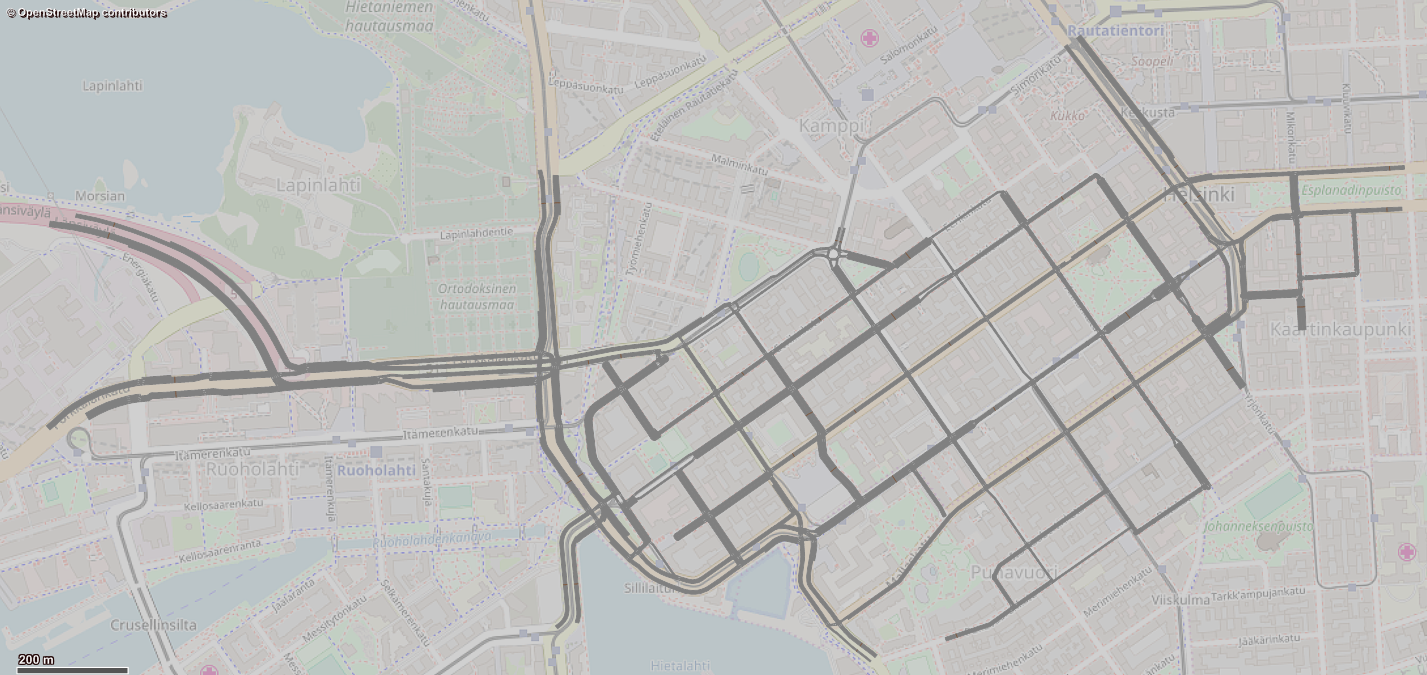
\includegraphics[width=0.75\textwidth]{graphs/vissim_map}
    \caption{The simulation area. Simulation roads shown with dark gray. Background map by OpenStreetMap\cite{osm}.}
\end{figure}

\subsection{Traffic}

After the map data was prepared, traffic inputs and sinks were defined for the simulation. Several entry and exit points for vehicles were placed at roads that enter or leave the simulation area. The dynamic traffic assignment in Vissim models traffic by using traffic demand data for the entry and exit points of the network. In the simulation, traffic demand data was supplied using a demand matrix (i.e. a matrix with $n$ columns and $m$ rows, where $n$ is the number of exit points, $m$ is the number of entry points and the column $i$ on the row $j$ is the flow rate from entry point $j$ to exit point $i$).

At first, these flow rates were simply estimated. However, the realism of the simulation is greatly dependant on having realistic traffic data and the validity of measurements based on this sort of data would be dubious. The demand values were refined with real-life road usage data from the area, published by the Helsinki Urban Environment Division \cite{trafficamounts}. Data for the biggets roads that were assigned as entry or exit points could be found in the dataset, but some had to be estimated. Traffic amounts between 8:00 and 9:00 were chosen, therefore the simulation should represent the morning commute period.

TODO: weaknesses and unrealistic aspects of the setup. All traffic is passing through

\begin{figure}[h]
    \centering
    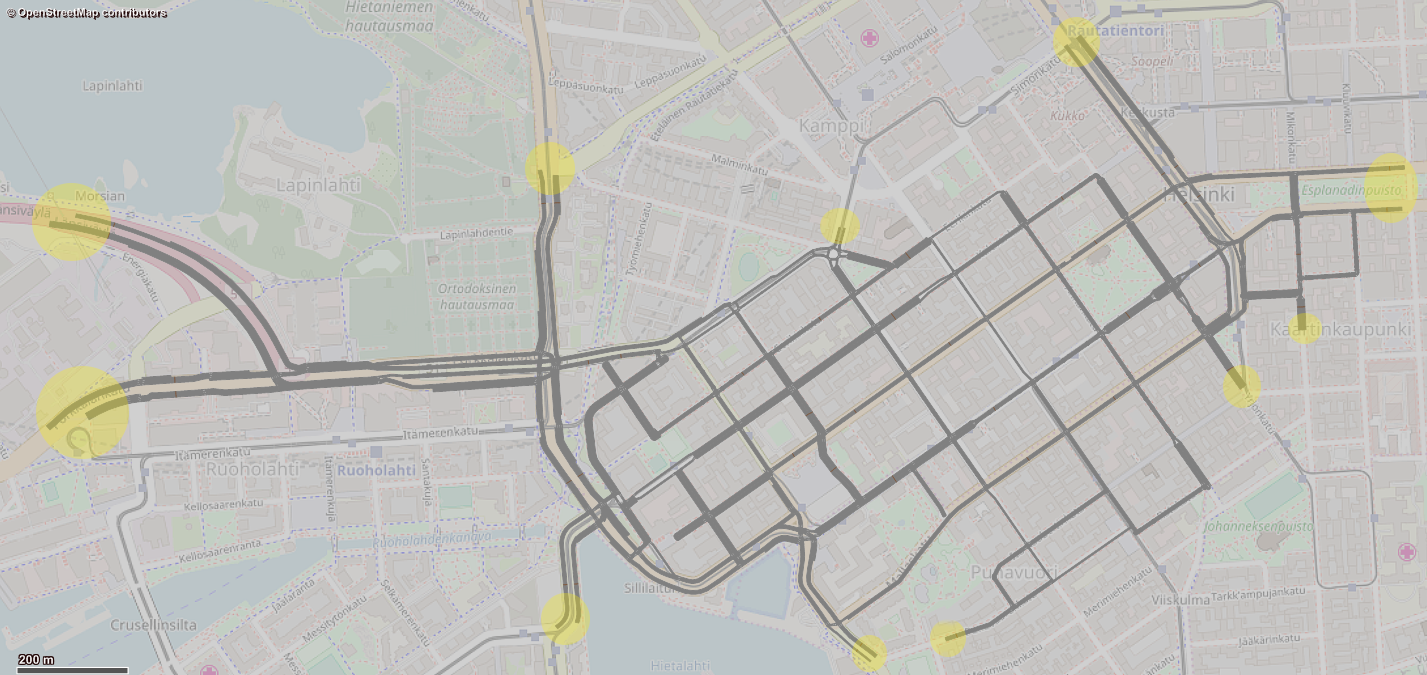
\includegraphics[width=0.75\textwidth]{graphs/vissim_map_entries}
    \caption{The simulation area. Exit and entry points highlighted with yellow. Background map by OpenStreetMap\cite{osm}.}
\end{figure}

\subsection{Data collection}

To analyze the macroscopic behavior of the simulation, the flow rate and the velocity of traffic should be measured from the simulation, as mentioned in the background section. Vissim features data collection points that can be placed on the and that automatically record the flow rate and the average velocity of traffic for the point in time periods of configurable length. Data collection points were placed several points in the simulation network. 

After running the simulation, data for flow rate and average velocity could be measured for each measurement period. Based on the flow rate and velocity, traffic density could be calculated. Based on these quantities, an analysis of the network could be carried out.

\subsection{Running the simulation}

To run the simulation, Vissim's Component Object Model (COM) interface was used. The COM interface is an inter-process communication method. The Python programming language and the pywin32 library was used to interface with Vissim via the COM interface. This allowed for automated repeated runs of the simulation while varying parameters between runs. Collecting traffic data from Vissim was also done via the Python code and the collected data was visualized with matplotlib and its plotting functionality. All used code can be found in Appendix A.

Each iteration of the simulation is run for 10 simulation minutes. Also the traffic demand is changed between each iteration by multiplying each cell of the demand matrix by a number, ranging from $0.5$ to $2.0$. We run a total of 8 rounds of simulation, collecting traffic data for each run. When all the runs have been done, we draw flow-density and speed-density diagrams and also time-series plots for all the separate simulation runs for flow rate and velocity.

TODO: rewrite the previous paragraph properly

\clearpage

\section{Results}

TODO: Write this properly

After running the simulations, we get the following figures for Länsiväylä.

\begin{figure}[h]
    \centering
    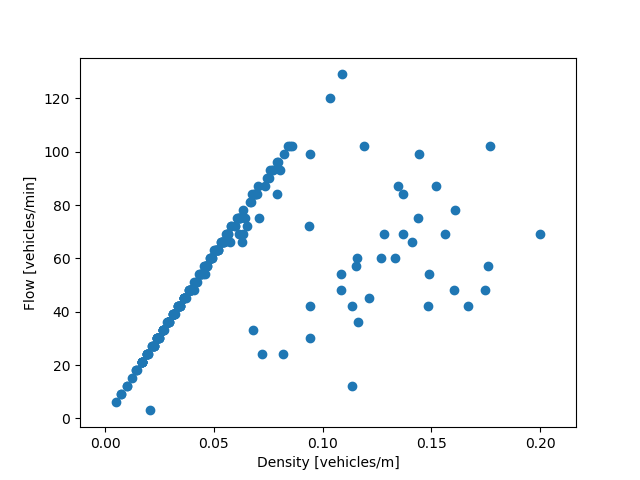
\includegraphics[width=0.75\textwidth]{graphs/Länsiväylä_2_flw_dns.png}
\end{figure}

\begin{figure}[h]
    \centering
    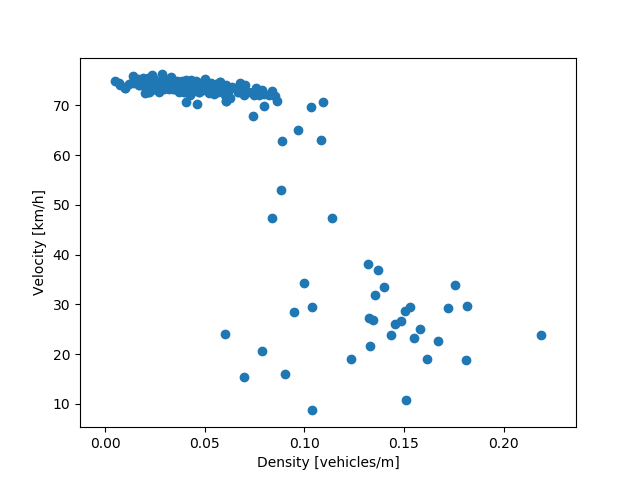
\includegraphics[width=0.75\textwidth]{graphs/Länsiväylä_2_spd_dns.png}
\end{figure}
\begin{figure}[h]
    \centering
    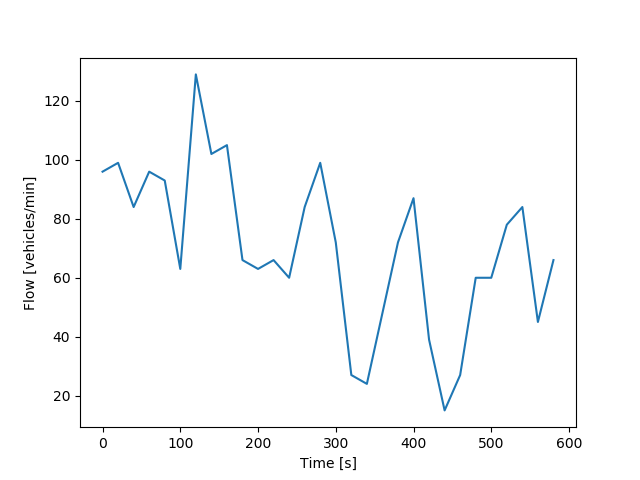
\includegraphics[width=0.75\textwidth]{graphs/Länsiväylä_2_flw_time_8.png}
\end{figure}

\begin{figure}[h]
    \centering
    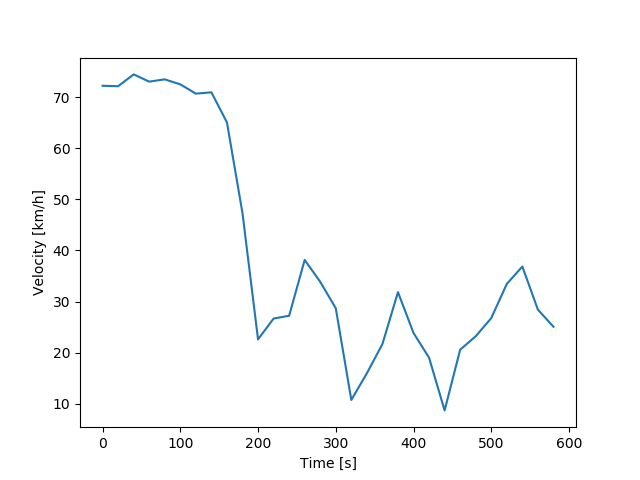
\includegraphics[width=0.75\textwidth]{graphs/Länsiväylä_2_spd_time_8.png}
\end{figure}

From the flow-density plot, we can see that during the simulation, the area reaches the S phase of the three-phase model. Also from the flow rate and velocity time-series plots we can see that at the pictured runs it reaches the J phase too.

TODO: do this for all interesting data collection points, not just Länäri

\subsection{Simulation results}

TODO: Examine simulation outcomes


\clearpage

\section{Summary}

TODO: Write this properly

As can be seen, there are bottlenecks in the network. Congestion pricing has been shown to reduce congestion in the critical road sections. That is one possible solution.

\clearpage

\thesisbibliography

\bibliography{bibliography}{}
\bibliographystyle{ieeetr}

\clearpage

\thesisappendix

\section{Python code}

Below is the Python code used to run the simulation and collect data. Running the code requires the Python libraries matplotlib and pywin32. The code is run by simply running \begin{verbatim}python main.py\end{verbatim}

\begin{verbatim}main.py\end{verbatim}
\lstinputlisting[language=Python]{code/main.py}

\begin{verbatim}simulation.py\end{verbatim}
\lstinputlisting[language=Python]{code/simulation.py}

\begin{verbatim}datacollector.py\end{verbatim}
\lstinputlisting[language=Python]{code/datacollector.py}

\begin{verbatim}figure.py\end{verbatim}
\lstinputlisting[language=Python]{code/figure.py}

\begin{verbatim}settings.py\end{verbatim}
\lstinputlisting[language=Python]{code/settings.py}

\end{document}
